% Editable source for the method overview in main.tex.
% Build from this directory: pdflatex -interaction=nonstopmode approach.tex
\documentclass[tikz,border=2pt]{standalone}
\usepackage{amsmath,amssymb}
\usepackage{tikz}
\usetikzlibrary{arrows.meta,calc,positioning,shapes.geometric}
\definecolor{ink}{HTML}{253449}
\definecolor{muted}{HTML}{657386}
\definecolor{blue}{HTML}{3069A8}
\definecolor{bluebg}{HTML}{EAF2FA}
\definecolor{orange}{HTML}{B76523}
\definecolor{orangebg}{HTML}{FFF0DE}
\definecolor{teal}{HTML}{168079}
\definecolor{tealbg}{HTML}{E1F3F0}
\definecolor{purple}{HTML}{7455A1}
\definecolor{purplebg}{HTML}{F0EBF7}
\definecolor{red}{HTML}{C44949}
\tikzset{
  every picture/.style={font=\sffamily},
  panel/.style={draw=ink!50,rounded corners=3pt,line width=.55pt,fill=white},
  flow/.style={-{Latex[length=2.1mm,width=1.35mm]},draw=ink,line width=.75pt},
  lightflow/.style={-{Latex[length=1.7mm,width=1.1mm]},draw=muted,line width=.55pt},
  paneltitle/.style={font=\sffamily\bfseries\fontsize{8}{9}\selectfont,text=ink,anchor=west},
  small/.style={font=\sffamily\fontsize{6.9}{8}\selectfont,text=ink,align=center},
  tinylabel/.style={font=\sffamily\fontsize{6.1}{7}\selectfont,text=muted,align=center},
  graphnode/.style={circle,draw=purple,fill=purplebg,inner sep=0pt,minimum size=3.5mm,line width=.55pt},
  frame/.style={draw=blue,fill=bluebg,rounded corners=1pt,minimum width=.69cm,minimum height=.48cm},
}
\begin{document}
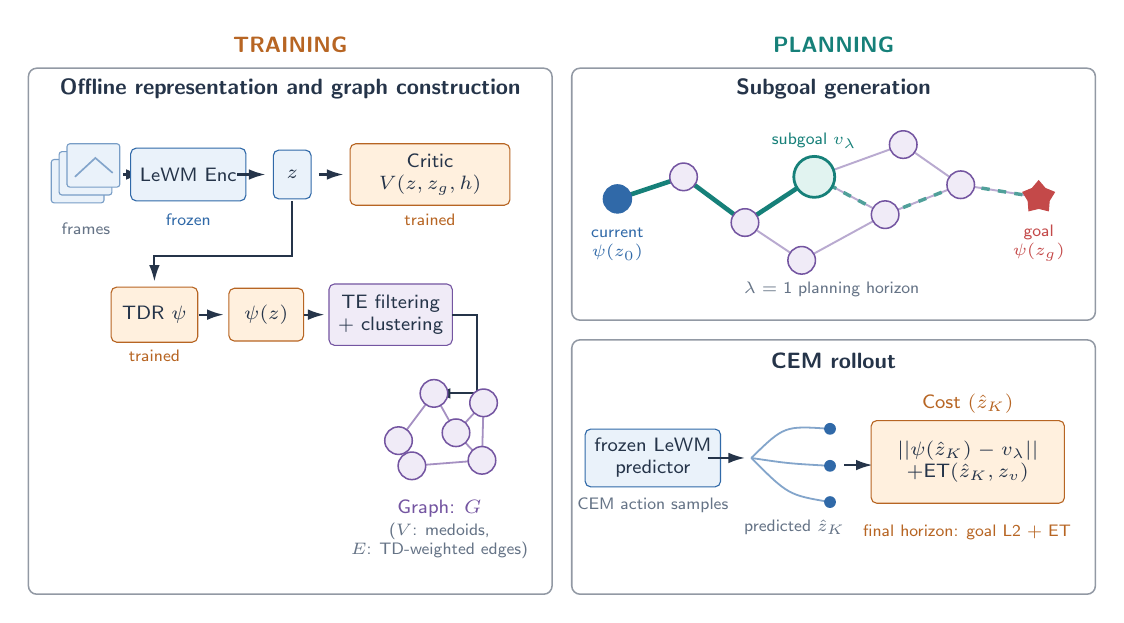
\begin{tikzpicture}[x=1cm,y=1cm]
  % Training-time stages are on the left; evaluation-time stages are on the right.
  % The outer dimensions are 13.55 x 7.12 cm, suitable for an ICLR text column.
  \node[font=\sffamily\bfseries\fontsize{8.4}{9}\selectfont,text=orange] at (3.325,6.98) {TRAINING};
  \node[font=\sffamily\bfseries\fontsize{8.4}{9}\selectfont,text=teal] at (10.225,6.98) {PLANNING};
  \draw[panel] (0,0) rectangle (6.65,6.68);
  \draw[panel] (6.9,3.48) rectangle (13.55,6.68);
  \draw[panel] (6.9,0) rectangle (13.55,3.23);

  % Training: the frozen encoder produces z. The critic branches right from z;
  % TDR starts the lower left-to-right representation-to-graph chain.
  \node[paneltitle,anchor=center] at (3.325,6.42) {Offline representation and graph construction};
  \foreach \dx/\dy in {0/.00,.10/.10,.20/.20} {
    \draw[fill=bluebg,draw=blue!65,rounded corners=1pt] (.29+\dx,4.97+\dy) rectangle (.96+\dx,5.52+\dy);
    \draw[blue!60,line width=.6pt] (.39+\dx,5.10+\dy) -- (.65+\dx,5.34+\dy) -- (.87+\dx,5.15+\dy);
  }
  \node[tinylabel] at (.73,4.64) {frames};
  \draw[flow] (1.20,5.33) -- (1.45,5.33);
  \node[draw=blue,fill=bluebg,rounded corners=2pt,small,minimum width=1.18cm,minimum height=.67cm] at (2.03,5.33) {LeWM Enc};
  \node[tinylabel,text=blue] at (2.03,4.76) {frozen};
  \draw[flow] (2.65,5.33) -- (3.01,5.33);
  \node[draw=blue,fill=bluebg,rounded corners=2pt,small,minimum width=.48cm,minimum height=.62cm] at (3.35,5.33) {$z$};
  \draw[flow] (3.69,5.33) -- (4.00,5.33);
  \node[draw=orange,fill=orangebg,rounded corners=2pt,small,minimum width=2.03cm,minimum height=.78cm] at (5.10,5.33) {Critic\\$V(z,z_g,h)$};
  \node[tinylabel,text=orange] at (5.10,4.75) {trained};

  \draw[flow] (3.35,4.99) -- (3.35,4.30) -- (1.60,4.30) -- (1.60,3.97);
  \node[draw=orange,fill=orangebg,rounded corners=2pt,small,minimum width=1.10cm,minimum height=.70cm] at (1.60,3.55) {TDR $\psi$};
  \node[tinylabel,text=orange] at (1.60,3.03) {trained};
  \draw[flow] (2.16,3.55) -- (2.48,3.55);
  \node[draw=orange,fill=orangebg,rounded corners=2pt,small,minimum width=.95cm,minimum height=.67cm] at (3.02,3.55) {$\psi(z)$};
  \draw[flow] (3.50,3.55) -- (3.76,3.55);
  \node[draw=purple,fill=purplebg,rounded corners=2pt,small,minimum width=1.54cm,minimum height=.78cm] at (4.60,3.55) {TE filtering\\+ clustering};
  \draw[flow] (5.38,3.55) -- (5.70,3.55) -- (5.70,2.55) -- (5.15,2.55);
  \coordinate (a) at (4.70,1.95); \coordinate (b) at (5.15,2.55);
  \coordinate (c) at (5.43,2.05); \coordinate (d) at (5.78,2.43);
  \coordinate (e) at (5.76,1.70); \coordinate (f) at (4.87,1.63);
  \foreach \u/\v in {a/b,b/c,c/d,d/e,c/e,a/f,f/e} \draw[purple!65,line width=.65pt] (\u) -- (\v);
  \foreach \n in {a,b,c,d,e,f} \node[graphnode] at (\n) {};
  \node[small,text=purple] at (5.22,1.08) {Graph: $G$};
  \node[tinylabel] at (5.22,.68) {($V$: medoids, \\ $E$: TD-weighted edges)};

  % Planning: online route selection, explicitly one CEM horizon ahead.
  \node[paneltitle,anchor=center] at (10.225,6.42) {Subgoal generation};
  \begin{scope}[shift={(6.9,3.48)}]
    \coordinate (s) at (.58,1.54); \coordinate (g1) at (1.42,1.82);
    \coordinate (g2) at (2.20,1.24); \coordinate (g3) at (3.08,1.82);
    \coordinate (g4) at (3.98,1.34); \coordinate (g5) at (4.94,1.72);
    \coordinate (goal) at (5.93,1.56); \coordinate (low) at (2.92,.76);
    \coordinate (upper) at (4.21,2.23);
    \foreach \u/\v in {s/g1,g1/g2,g2/g3,g3/g4,g4/g5,g5/goal,g2/low,low/g4,g3/upper,upper/g5} \draw[purple!50,line width=.7pt] (\u) -- (\v);
    \draw[teal,line width=1.65pt,-{Latex[length=1.6mm]}] (s) -- (g1) -- (g2) -- (g3);
    \draw[teal!75,line width=1.25pt,dashed] (g3) -- (g4) -- (g5) -- (goal);
    \foreach \n in {g1,g2,g4,g5,low,upper} \node[graphnode] at (\n) {};
    \node[circle,draw=blue,fill=blue,inner sep=0pt,minimum size=3.6mm] at (s) {};
    \node[circle,draw=teal,fill=tealbg,inner sep=0pt,minimum size=5.2mm,line width=1pt] at (g3) {};
    \node[star,star points=5,draw=red,fill=red,inner sep=0pt,minimum size=4.2mm] at (goal) {};
    \node[tinylabel,text=blue] at (.58,.96) {current \\ $\psi(z_0)$};
    \node[tinylabel,text=teal] at (3.08,2.28) {subgoal $v_\lambda$};
    \node[tinylabel,text=red] at (5.93,.98) {goal \\ $\psi(z_g)$};
    \node[tinylabel] at (3.30,.39) {$\lambda=$ 1 planning horizon};
  \end{scope}

  % One unchanged low-level controller; only the terminal ranking changes.
  \node[paneltitle,anchor=center] at (10.225,2.97) {CEM rollout};
  \begin{scope}[shift={(6.9,0)}]
    \node[draw=blue,fill=bluebg,rounded corners=2pt,small,minimum width=1.34cm,minimum height=.70cm] at (1.03,1.73) {frozen LeWM\\predictor};
    \node[tinylabel] at (1.03,1.13) {CEM action samples};
    \draw[flow] (1.73,1.73) -- (2.20,1.73);
    \coordinate (root) at (2.28,1.73);
    \draw[blue!60,line width=.65pt] (root) .. controls (2.70,2.14) .. (3.28,2.10);
    \draw[blue!60,line width=.65pt] (root) .. controls (2.75,1.66) .. (3.28,1.63);
    \draw[blue!60,line width=.65pt] (root) .. controls (2.75,1.26) .. (3.28,1.17);
    \foreach \x/\y in {3.28/2.10,3.28/1.63,3.28/1.17} \fill[blue] (\x,\y) circle (.075);
    \node[tinylabel] at (2.83,.85) {predicted $\hat z_K$};
    \draw[flow] (3.46,1.64) -- (3.82,1.64);
    \node[small,text=orange] at (5.03,2.42) {Cost $(\hat z_K)$};
    \node[draw=orange,fill=orangebg,rounded corners=2pt,small,text width=2.22cm,minimum height=1.05cm] at (5.03,1.68) {$|| \psi(\hat z_K) - v_\lambda ||$ $+ \text{ET}(\hat z_K, z_v ) $};
    \node[tinylabel,text=orange] at (5.02,.79) {final horizon: goal L2 $+$ ET};
  \end{scope}
\end{tikzpicture}
\end{document}
